% !TEX root = MMAM_ST.tex
% This work is licensed under the Creative Commons
% Attribution-NonCommercial-ShareAlike 4.0 International License. To view a copy
% of this license, visit http://creativecommons.org/licenses/by-nc-SA/4.0/ or
% send a letter to Creative Commons, PO Box 1866, Mountain View, CA 94042, USA.

\section*{Organisatorisches}%
\label{sec:Organisatorisches}

Bei Fragen während der Vorlesungs- und Prüfungsphase:

Email: schwartz@gsc.tu-darmstadt.de

Diese Information wird nur für die oben genannte Zeitspanne im Skript enthalten bleiben.

\chapter{Einführung}

\section{Beispiele}%
\label{sec:Beispiele}

\begin{definition}
	Ein \underline{strategisches Spiel in Normalform} besteht aus 
	\begin{itemize}
		\item eine Menge von \underline{Spielern}  $i=1,\ldots, N$
		\item zulässige \underline{Strategiemengen} $X_i, \quad i=1,\ldots, N$
		\item \underline{Auszahlungsfunktionen}  $f_i : \underbrace{X_1 \times \ldots \times X_N}_{:=X} \to \R$
	\end{itemize}
	\underline{Problem} von Spieler i:
	\begin{itemize}
		\item $\min\limits_{x_i} f_i(x_1, \ldots, x_i, \ldots, x_N)$ mit $x_i \in X_i$
	\end{itemize}
\end{definition}

\begin{beispiel}
	(Schere, Stein, Papier)
	\begin{itemize}
		\item zwei Spieler : $i=1,2$
		\item Strategiemengen : $X_1 = X_2 = \left\{\text{Schere, Stein, Papier}\right\}$
		\item Auszahlungsfunktion : (Wer verliert, zahlt 1€ an den Gegner)

			Auszahlung für Spieler 1:
			\[
				f_1(x_1,x_2) = \begin{cases}
					\hfil -1 &\quad x_1 = \text{Schere}, x_2 =\text{Stein} \\
					\hfil +1 &\quad x_1 = \text{Schere}, x_2 = \text{Papier} \\
					\hfil 0 &\quad x_1 = \text{Schere}, x_2 = \text{Schere} \\
					\hfil \vdots &\quad \hfil \vdots
				\end{cases}
			\] 
			Auszahlung für Spieler 2:
			\[
				f_2(x_1,x_2) = \begin{cases}
					\hfil +1 &\quad x_1 = \text{Schere}, x_2 =\text{Stein} \\
					\hfil -1 &\quad x_1 = \text{Schere}, x_2 = \text{Papier} \\
					\hfil 0 &\quad x_1 = \text{Schere}, x_2 = \text{Schere} \\
					\hfil \vdots &\quad \hfil \vdots
				\end{cases}
			\]
			\begin{center}
				\begin{tabular}{cc|c|c|c|}
					\\ \cline{3-5}
					&&\multicolumn{3}{c|}{{\color{red} Spieler 1}} \\ \cline{3-5}
					&&Schere &Stein & Papier \\ \hline
					\multicolumn{1}{ |c }{\multirow{3}{*}{\color{blue} Spieler 2}}&
					\multicolumn{1}{ |c| }{Schere} & \color{blue}0\color{black},\color{red} 0 & \color{blue}-1\color{black},\color{red} +1 & \color{blue}+1\color{black},\color{red} -1 \\ \cline{2-5}
					\multicolumn{1}{ |c }{}&
					\multicolumn{1}{ |c| }{Stein} & \color{blue}+1\color{black},\color{red} -1 & \color{blue}0\color{black},\color{red} 0 & \color{blue}-1\color{black},\color{red} +1 \\ \cline{2-5}
					\multicolumn{1}{ |c }{}&
					\multicolumn{1}{ |c|}{Papier} & \color{blue}-1\color{black},\color{red} +1 & \color{blue}+1\color{black},\color{red} -1 & \color{blue}0\color{black},\color{red} 0  \\ \hline
				\end{tabular}
			\end{center}
	\end{itemize}
\end{beispiel}

\begin{beispiel}
	(Gefangenendilemma):

	Angebot des Staatsanwalts:
	\begin{itemize}
		\item Verdächtiger gesteht, aber Partner schweigt:

			Geständiger muss nur 1 Jahr ins Gefängnis

			Schweigender Partner muss 10 Jahre ins Gefängnis
		\item Wenn beide gestehen:
			
			Beide müssen für 5 Jahre ins Gefängnis
		\item Wenn keiner gesteht:
			
			Beide müssen wegen anderer Vergehen für 2 Jahre ins Gefängnis
	\end{itemize}
	\[
	\implies
	\] 
	\begin{itemize}
		\item Spieler : $i=1, 2$
		\item Strategiemengen : $X_1 = X_2 = \{\text{schweigen, gestehen}\}$
	\end{itemize}
	\begin{center}
		\begin{tabular}{cc|c|c|}
			\\ \cline{3-4}
			&&\multicolumn{2}{c|}{{\color{red} Spieler 1}} \\ \cline{3-4}
			&&schweigen &gestehen \\ \hline
			\multicolumn{1}{ |c }{\multirow{2}{*}{\color{blue} Spieler 2}}&
			\multicolumn{1}{ |c| }{schweigen} & \color{blue}2\color{black},\color{red} 2 & \color{blue}10\color{black},\color{red} 1 \\ \cline{2-4}
			\multicolumn{1}{ |c }{}&
			\multicolumn{1}{ |c| }{gestehen} & \color{blue}1\color{black},\color{red} 10 & \color{blue}5\color{black},\color{red} 5 \\ \hline
		\end{tabular}
	\end{center}
\end{beispiel}

\begin{beispiel}
	(Koordinationsspiel, Kampf der Geschlechter)
	\begin{itemize}
		\item 2 Spieler : $i = 1, 2$
		\item Strategiemengen : $X_1 = X_2 = \{\text{A, B}\}$
			hierbei sind $A$ und $B$ z.B. die von den jeweiligen Spielern bevorzugten Aktivitäten (explizites Beispiel: $A$ = in die Oper gehen vs. $B$ = zum Fußballspiel gehen)
			\begin{center}
				\begin{tabular}{cc|c|c|}
					\\ \cline{3-4}
					&&\multicolumn{2}{c|}{{\color{red} Spieler 1}} \\ \cline{3-4}
					&&A &B \\ \hline
					\multicolumn{1}{ |c }{\multirow{2}{*}{\color{blue} Spieler 2}}&
					\multicolumn{1}{ |c| }{A} & \color{blue}2\color{black},\color{red} 1 & \color{blue}0\color{black},\color{red} 0 \\ \cline{2-4}
					\multicolumn{1}{ |c }{}&
					\multicolumn{1}{ |c| }{B} & \color{blue}0\color{black},\color{red} 0 & \color{blue}1\color{black},\color{red} 2 \\ \hline
				\end{tabular}
			\end{center}

	\end{itemize}
	Auszahlungen werden bei "Schere-Stein-Papier" und dem "Kampf der Geschlechter" in diesen Beispielen im Gegensatz zum Normalfall maximiert!
\end{beispiel}

\begin{beispiel}
	(Cournot-Oligopol)

	Firmen $F_i, \quad i=1,\ldots,N$ stellen das gleiche
	Gut her. Die Produktion von $x_i$ Einheiten kostet
	$c_i(x_i)$ für Firma $F_{i}$. Der Preis fällt mit dem Gesamtangebot, d.h.
	$p(\sum_{i=1}^{N} x_i)$.
	Das Problem der Firma ist, den Gewinn zu maximieren:
	\[
		\max\limits_{x_i} p(\sum_{j=1}^N x_j)\cdot x_i - c_i(x_i) \qquad \mit x_i \geq 0 \quad\text{(+ weitere Restriktionen)}
	.\] 
\end{beispiel}

\section{Klassifikation von Spielen}%
\label{sec:Klassifikation von Spielen}

Wir werden nun Spiele nach unterschiedlichen Kriterien charakterisieren und einige Definitionen einführen.

\begin{definition} (Charakterisierung nach Auszahlungsfunktion)

	Ein Spiel $\Gamma=\{X_i, f_i\}_{i=1}^N$ heißt
	\begin{itemize}
		\item \underline{Nullsummenspiel}, wenn gilt
			\[
				\sum_{i=1}^N f_i(x_1, \ldots, x_N)=0 \qquad \forall (x_1, \ldots, x_N) \in X
			.\] 
		\item \underline{Konstantsummenspiel}, wenn gilt
			\[
				\sum_{i=1}^N f_i(x_1, \ldots, x_N)=c \qquad \forall (x_1, \ldots, x_N) \in X
			.\] 
		\item \underline{Nichtnullsummenspiel}, wenn es kein Konstantsummenspiel ist.
	\end{itemize}
\end{definition}

\begin{definition} (Charakterisierung nach Größe der Strategiemengen) 

	Ein Spiel $\Gamma=\{X_i, f_i\}_{i=1}^N$ heißt
	\begin{itemize}
		\item \underline{endlich}, wenn alle Strategiemengen $X_i$ nur endlich viele Elemente haben.
		\item \underline{abzählbar}, wenn alle Strategiemengen $X_i$ abzählbar viele Elemente haben
		\item \underline{überabzählbar} oder \underline{kontinuierlich}, in allen andern Fällen
	\end{itemize}
\end{definition}

\begin{definition} (Charakterisierung nach Anzahl der Spieler)
	\begin{itemize}
		\item Ein endliches 2-Personen-Spiel heißt \underline{Bi-Matrixspiel} 
		\item Ein endliches 2-Personen-Nullsummenspiel heißt \underline{Matrixspiel} 
	\end{itemize}
\end{definition}

\begin{beispiel}
	(Endliches 2-Personen-Spiel)
	\begin{align*}
		X_1 = \{a_1, a_2, \ldots, a_m\} \text{ durchnummerieren } \rightarrow \quad X=\{1,\ldots,m\} \\
		X_2 = \{b_1, b_2, \ldots, b_n\} \text{ durchnummerieren } \rightarrow \quad X=\{1,\ldots,n\} 
	\end{align*}
Auszahlungsmatrizen für Spieler 1 und 2: \[A, B \in R^{m \times n} \mit a_{ij} = f_1(a_i, b_j), \quad b_{ij} = f_2(a_i, b_j)
.\]

Damit dieses Spiel ein Nullsummenspiel ist, müsste gelten \[
B = -A
.\] 
\end{beispiel}

Weitere zahlreiche Unterscheidungsmöglichkeiten von Spielen
\begin{itemize}
	\item kooperativ oder \underline{nichtkooperativ} 
	\item \underline{einmaliges} oder wiederholbares Spiel
	\item \underline{vollständige} versus unvollständige Information
	\item \underline{simultane} oder sequentielle Entscheidungen
\end{itemize}

Um in den folgenden Kapiteln die Notation zu vereinfachen, treffen wir die folgenden Konventionen:

\begin{itemize}
	\item Vektor aller Strategien : $x = (x_1^{T},x_2^{T}, \ldots, x_{N}^{T})^{T}$
	\item Blickwinkel von Spieler i :
		\begin{itemize}
			\item eigene Strategie : $x_{i}$
			\item gegnerische Strategien $x_{-i} = (x_1, \ldots, x_{i-1}, x_{i+1}, \ldots, x_{N})$

		\end{itemize}
		Damit gilt $x = (x_{i}, x_{-i})$
	\item Vektor : $(x_1, \ldots, x_{i-1}, x_{i}^{*}, x_{i+1}, \ldots, x_{N}) = (x_{i}^{*}, x_{-i})$
\end{itemize}

\begin{definition}
	Betrachte ein Spiel $\Gamma=\{X_{i}, f_{i}\}_{i=1}^{N}$.
	Dann heißt eine Strategiekombination $x^{*} = (x_1^{*}, \ldots, x_{N}^{*})$ ein \underline{Nash-Gleichgewicht} von $\Gamma$, wenn gilt:
	\begin{enumerate}
		\item $x_{i}^{*} \in X_{i} \quad \forall i=1, \ldots, N$
		\item $f_{i}(x_{i}^{*}, x_{-i}^{*}) \leq f_{i}(x_{i}, x_{-i}^{*}) \quad \forall x_{i} \in X_{i} \forall i=1, \ldots, N$
	\end{enumerate}
\end{definition}

\begin{definition}
	Betrachte ein Spiel $\Gamma=\{X_{i}, f_{i}\}_{i=1}^{N}$.
	Für ein gegebenes $x_{-i} \in X_{-i} := X_1 \times \ldots \times X_{i-1} \times X_{i+1} \times \ldots \times X_{N}$ ist die \underline{Beste Antwort} von Spieler $i$ definiert als
	\[
		S_{i}(x_{-i}) = \argmin\limits_{x_{i}}\{f_{i}(x_{i}, x_{-i}) | x_{i} \in X_{i}\}
	.\] 
	Die Abbildung $S: X \rightrightarrows X$ mit 
	\[
		S(x) = S_1(x_{-1}) \times \ldots \times S_{N}(x_{-N})	
	.\] 
	heißt \underline{Beste-Antwort-Funktion} des Spiels.
\end{definition}

\begin{satz}
	$x^{*}$ ist ein Nash-Gleichgewicht des Spiels $\Gamma=\{X_{i}, f_{i}\}_{i=1}^{N}$ genau dann, wenn gilt
	\[
		x^{*} \in S(x^{*})
	.\] 
\end{satz}

Als nächstes Betrachten wir noch einmal unsere drei Beispiele und untersuchen sie auf Nash-Gleichgewichte:

\begin{figure}[ht!]
\centering
\begin{subfigure}[b]{\textwidth}
\begin{center}
	\begin{tabular}{cc|c|c|c|}
		\\ \cline{3-5}
		&&\multicolumn{3}{c|}{{\color{red} Spieler 1}} \\ \cline{3-5}
		&&Schere &Stein & Papier \\ \hline
		\multicolumn{1}{ |c }{\multirow{3}{*}{\color{blue} Spieler 2}}&
		\multicolumn{1}{ |c| }{Schere} & 0, 0 & -1, \cunderline{red}{+1} & \cunderline{blue}{+1}, -1 \\ \cline{2-5}
		\multicolumn{1}{ |c }{}&
		\multicolumn{1}{ |c| }{Stein} & \cunderline{blue}{+1}, -1 & 0, 0 & -1, \cunderline{red}{+1} \\ \cline{2-5}
		\multicolumn{1}{ |c }{}&
		\multicolumn{1}{ |c|}{Papier} & -1, \cunderline{red}{+1} & \cunderline{blue}{+1}, -1 & 0, 0  \\ \hline
	\end{tabular}
\caption{Hat keine Nash-Gleichgewichte}
\label{fig:Bsp1NashGG}
\end{center}
\end{subfigure}

\begin{subfigure}[b]{\textwidth}
\begin{center}
	\begin{tabular}{cc|c|c|}
		\\ \cline{3-4}
		&&\multicolumn{2}{c|}{{\color{red} Spieler 1}} \\ \cline{3-4}
		&&schweigen &gestehen \\ \hline
		\multicolumn{1}{ |c }{\multirow{2.75}{*}{\color{blue} Spieler 2}}&
		\multicolumn{1}{ |c| }{schweigen} & 2, 2 & 10, \cunderline{red}{1} \\ \cline{2-4}
		\multicolumn{1}{ |c }{}&
		\multicolumn{1}{ |c| }{gestehen} & \cunderline{blue}{1}, 10 & \tikz [anchor=base, baseline] \node[ellipse,draw,color=black,text=black] {\cunderline{blue}{5}, \cunderline{red}{5}}; \\ \hline
	\end{tabular}
\caption{Hat ein Nash-Gleichgewicht}
\label{fig:Bsp2NashGG}
\end{center}
\end{subfigure}

\begin{subfigure}[b]{\textwidth}
\begin{center}
	\begin{tabular}{cc|c|c|}
		\\ \cline{3-4}
		&&\multicolumn{2}{c|}{{\color{red} Spieler 1}} \\ \cline{3-4}
		&&A &B \\ \hline
		\multicolumn{1}{ |c }{\multirow{2.75}{*}{\color{blue} Spieler 2}}&
		\multicolumn{1}{ |c| }{A} & \tikz [anchor=base, baseline] \node[ellipse,draw,color=black,text=black] {\cunderline{blue}{2}, \cunderline{red}{1}}; & 0, 0 \\ \cline{2-4}
		\multicolumn{1}{ |c }{}&
		\multicolumn{1}{ |c| }{B} & 0, 0 & \tikz [anchor=base, baseline] \node[ellipse,draw,color=black,text=black] {\cunderline{blue}{1}, \cunderline{red}{2}}; \\ \hline
	\end{tabular}
\caption{Hat mehrere Nash-Gleichgewichte}
\label{fig:Bsp3NashGG}
\end{center}
\end{subfigure}
\end{figure}

Beachte hier wieder, dass in den Fällen $(a)$ und $(c)$ die
Lösung ein Maximum sein soll und in $(b)$ ein Minimum sein
soll.

\begin{beispiel}(Cournot-Oligopol)

Problem von Spieler 1 : $\max\limits_{x_1} p(x_1 + x_2) \cdot x_1 - c_1(x_1) \qquad \mit x_1 \geq 0$ 

Problem von Spieler 2 : $\max\limits_{x_2} p(x_1 + x_2) \cdot x_2 - c_2(x_2) \qquad \mit x_2 \geq 0$ 

Annahmen:
\begin{align*}
	c_{i}(x_{i}) &= c_{i} \cdot x_{i}&  &\mit c_{i} > 0 \quad \forall i=1,2 \\
	p(x_1 + x_2) &= \begin{cases}
		p-(x_1 + x_2) &\qquad \text{ für } x_1 +x_2 \leq p \\
		0 &\qquad \text{ für } x_1 + x_2 > p
	\end{cases}& &\mit p > 0 
\end{align*}

Damit können wir die Auszahlungsfunktion von Spieler 1
aufschreiben
\begin{align*}
	f_1(x_1, x_2) &= (p-x_1 -x_2) x_1 - c_1x_1 \\
				  &= -x_1^2 + (p-x_2-c_1)x_1 \\
\end{align*}
und über den klassischen Ansatz der Analysis (Betrachten der Ableitung) das Maximum dieser Funktion finden
\begin{align*}
	&\nabla_{x_1} f_1(x_1,x_2) = -2x_1 +(p-c_1-x_2) \stackeq{!} 0 \\
	\implies &x_1 = \frac{p-c_1-x_2}{2} \\
	\implies &S_1(x_2) = \begin{cases}
		\frac{p-c_1-x_2}{2} &\text{ falls } x_2 \leq p-c_1 \\
		0 &\text{ sonst}
	\end{cases}
\end{align*}

\begin{figure}[ht!]
\begin{center}
	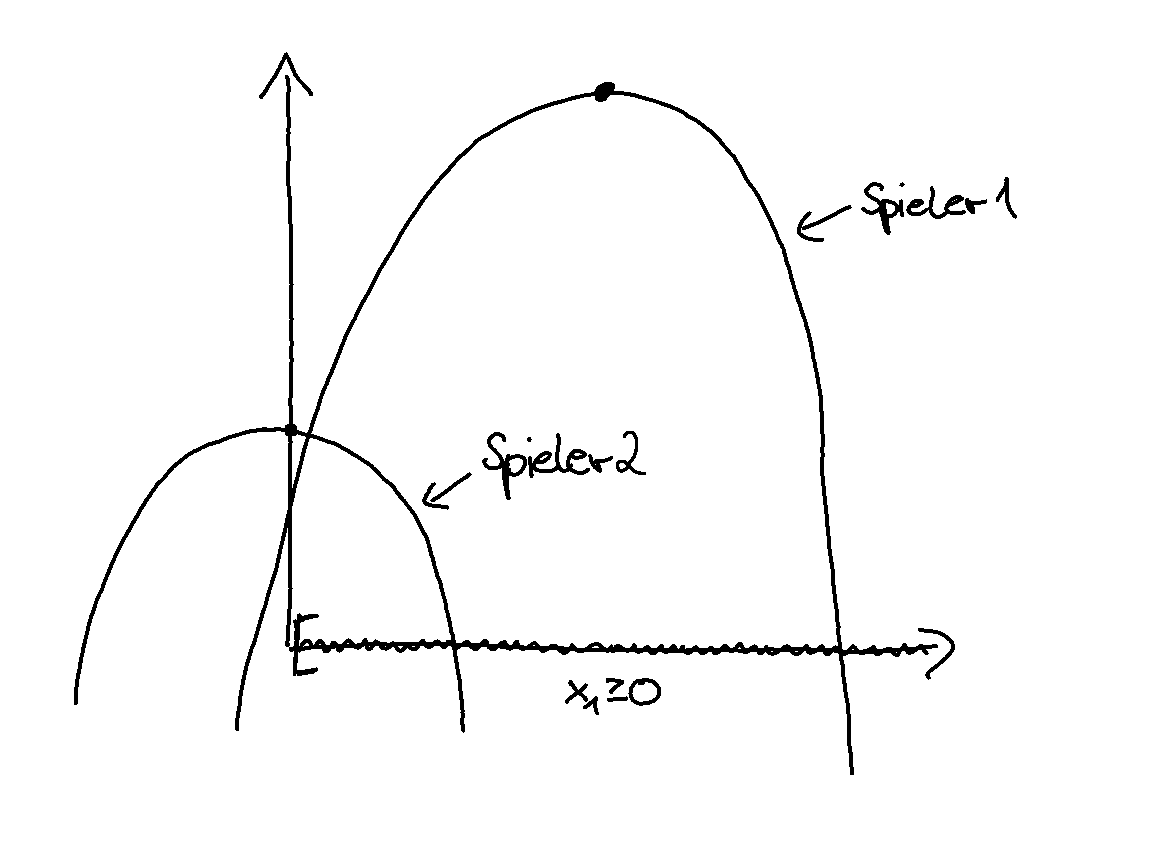
\includegraphics[scale=0.6]{pics/0.png}
\end{center}
\caption{Auszahlungsfunktionen aus dem Problem von Cournot-Oligopol}
\label{fig:CournotOligopolBsp_1}
\end{figure}

\begin{figure}[ht!]
\begin{center}
	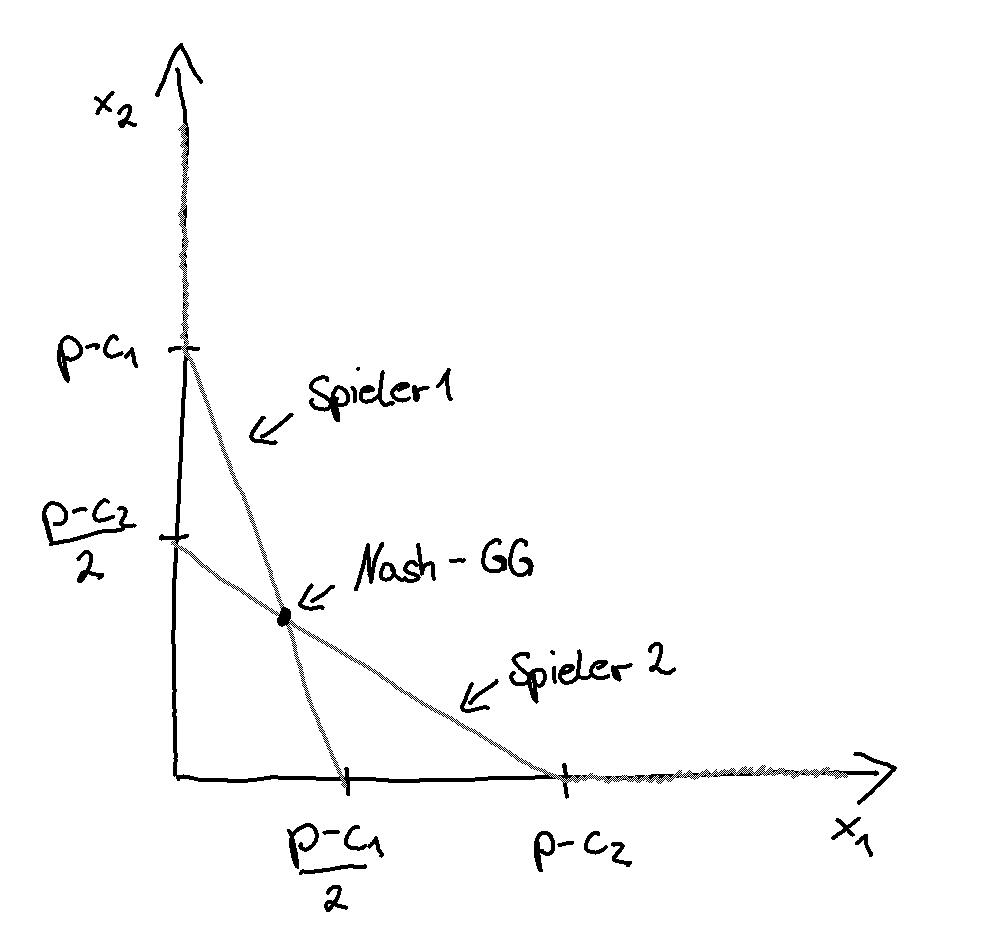
\includegraphics[scale=0.6]{pics/1.png}
\end{center}
\caption{Finden des Nash-Gleichgewichtes im Problem von Cournot-Oligopol}
\label{fig:CournotOligopolBsp_2}
\end{figure}
\end{beispiel}

\begin{satz}
	Betrachte zwei Spiele $\Gamma=\{X_{i}, f_{i}\}_{i=1}^{N}$ und $\tilde{\Gamma} = \{X_{i}, \tilde{f_{i}}\}$. Wenn gilt 
	\[
		\tilde{f_{i}}(x_{i},x_{-i}) = c_{i}f_{i}(x_{i}, x_{-i}) + r_{i}(x_{-i}) \qquad \mit c_{i} > 0
	.\] 
	für alle Spieler $i=1, \ldots, N$, so sind die Spiele \underline{strategisch equivalent}, d.h. besitzen die gleichen Nash-Gleichgewichte.
\end{satz}

\begin{satz}
	Jedes Konstantsummenspiel ist strategisch equivalent zu einem Nullsummenspiel.
\end{satz}

\begin{definition}
	Betrachte ein Spiel $\Gamma = \{X_{i}, f_{i}\}_{i=1}^{N}$.
	\begin{enumerate}[label=\alph{enumi})]
		\item Eine Strategie $x_{i}^{*}$ \underline{dominiert} $\tilde{x}_{i}$ strikt, wenn gilt
			\[
				f_{i}(x_{i}^{*}, x_{-i}) < f_{i}(\tilde{x}_{i}, x_{-i}) \qquad \forall x_{-i} \in X_{-i}
			.\] 
		\item Eine Strategie $x_{i}^{*}$ \underline{dominiert} $\tilde{x}_{i}$ schwach, wenn gilt
			\[
				f_{i}(x_{i}^{*}, x_{-i}) \leq f_{i}(\tilde{x}_{i}, x_{-i}) \qquad \forall x_{-i} \in X_{-i}
			.\] 
		\item $x_{i}^{*}$ ist \underline{strikt (schwach) dominant}, wenn sie alle anderen Strategien $\tilde{x}_{i} \in X_{i} \setminus \{x_{i}^{*}\}$ strikt (schwach) dominiert.
		\item Ein Vektor $x^{*} \in X$ heißt \underline{Gleichgewicht in strikt (schwach) dominanten Strategien}, wenn $x_{i}^{*}$ strikt (schwach) dominant ist für alle Spieler $i=1, \ldots, N$ 
	\end{enumerate}
\end{definition}

\begin{satz}
	Jedes Gleichgewicht in strikt (schwach) dominanten
	Strategien ist ein Nash-Gleich-gewicht.
\end{satz}

\begin{proof}
	Sei $x^{*} \in X$ ein Gleichgewicht in schwach dominanten Strategien, d.h. es gilt für alle $i=1, \ldots, N$:
	\begin{align*}
		&f_{i}(x_{i}^{*}, x_{-i}) \leq f_{i}(x_{i}, x_{-i})& &\forall x_{-i} \in X_{-i}, \forall x_{i} \in X_{i} \\
		\implies &f_{i}(x_{i}^{*}, x_{-i}^{*}) \leq f_{i}(x_{i}, x_{-i}^{*})& &\forall x_{i} \in X_{i} \\
		\implies &x^{*} \text{ist ein Nash-Gleichgewicht.}
	\end{align*}
\end{proof}

\begin{beispiel}(Elimination dominanter Strategien)

Wir betrachten hier der Einfachheit halber wieder ein Maximierungsproblem.
	\begin{center}
		\begin{tabular}{c|c c c}
			& $b_1$ & $b_2$ & $b_3$ \\ \hline
			$a_1$ & 0, 1 & 1, 0 & \tikz [anchor=base, baseline] \node[ellipse,draw,color=black,text=black] {1, 1}; \\
			$a_2$ & 1, 0 & 0, 1 & \tikz [anchor=base, baseline] \node[ellipse,draw,color=black,text=black] {1, 2};
		\end{tabular}
		$\underset{\substack{\\\text{Erste Elimination}}}{\Longrightarrow}$
		\begin{tabular}{c|c}
			& $b_3$ \\ \hline
			$a_1$ & 1, 1 \\
			$a_2$ & 1, 2
		\end{tabular}
	\end{center}
	Strategie $b_{3}$ dominiert sowohl $b_1$ (schwach) als auch $b_2$. Das heißt, das Wählen der Strategie $b_3$ ergibt für Spieler 1 immer die maximale Auszahlung. Da Spieler 1 die anderen Strategien nie wählen wird (wenn er auszahlungsorientiert handelt), können wir $b_1$ und $b_2$ aus der Tabelle entfernen.
	\begin{center}
		\begin{tabular}{c|c}
			& $b_3$ \\ \hline
			$a_1$ & 1, 1\\
			$a_2$ & \tikz [anchor=base, baseline] \node[ellipse,draw,color=black,text=black] {1, 2};
		\end{tabular}
		$\underset{\substack{\\\text{Zweite Elimination}}}{\Longrightarrow}$
		\begin{tabular}{c|c}
			 & $b_3$ \\ \hline
			$a_2$ & 1, 2
		\end{tabular}
	\end{center}
	Nun ergibt sich jedoch wieder eine Situation, in der eine Strategie dominant ist. Dieses Mal wird Spieler 2 immer $a_2$ wählen. Auch hier können wir noch einmal eine Elimination durchführen. Das nun noch verbliebene Nash-Gleichgewicht ist eins der zwei Nash-Gleichgewichte.
\end{beispiel}

\section{Mehrzieloptimierung}%
\label{sec:Mehrzieloptimierung}

Sei $f \colon \R^{n} \rightarrow \R^{m}$, eine Funktion und $X \subseteq \R^{n}$. Dann ist die Problemstellung der Mehrzieloptimierung
\[
	"\min\limits_{x}" f(x) \qquad \mit x \in X
.\] 

\begin{definition}
	Ein Vektor $x^{*} \in X$ heißt \underline{Paretro-Gleichgewicht}, wenn es \underline{keinen} Vektor $\tilde{x} \in X$ mit
	\begin{align*}
	f_{i}(\tilde{x}) \leq f_{i}(x^{*}) \qquad
	\forall i=1, \ldots, m \\
	\end{align*}
	,wobei $"<"$ für mindestens ein $ i \in \{1, \ldots, m\}$.
	Diese Definition kann auch auf Spiele $\Gamma = \{X_{i},f_{i}\}_{i=1}^{N}$ angewandt werden mit 
	\[
	X=X_1 \times \ldots \times X_{N} \text{ und }f(x) = \begin{pmatrix}
		f_1(x) \\
		\vdots \\
		f_{N}(x)
	\end{pmatrix}
	.\]

	Man kann sie interpretieren durch: Man findet keine Strategie, die mindestens besser für einen Spieler und gleich gut für alle anderen Spieler ist, als das Paretro-Gleichgewicht.
\end{definition}

\begin{figure}[ht!]
\centering
\begin{subfigure}[b]{\textwidth}
\begin{center}
	\begin{tabular}{cc|c|c|c|}
		\\ \cline{3-5}
		&&\multicolumn{3}{c|}{{\color{red} Spieler 1}} \\ \cline{3-5}
		&&Schere &Stein & Papier \\ \hline
		\multicolumn{1}{ |c }{\multirow{4.5}{*}{\color{blue} Spieler 2}}&
		\multicolumn{1}{ |c| }{Schere} & \tikz [anchor=base, baseline] \node[ellipse,draw,color=black,text=black] {0, 0}; & \tikz [anchor=base, baseline] \node[ellipse,draw,color=black,text=black] {-1, +1}; & \tikz [anchor=base, baseline] \node[ellipse,draw,color=black,text=black] {+1, -1}; \\ \cline{2-5}
		\multicolumn{1}{ |c }{}&
		\multicolumn{1}{ |c| }{Stein} & \tikz [anchor=base, baseline] \node[ellipse,draw,color=black,text=black] {+1, -1}; & \tikz [anchor=base, baseline] \node[ellipse,draw,color=black,text=black] {0, 0}; & \tikz [anchor=base, baseline] \node[ellipse,draw,color=black,text=black] {-1, +1}; \\ \cline{2-5}
		\multicolumn{1}{ |c }{}&
		\multicolumn{1}{ |c|}{Papier} & \tikz [anchor=base, baseline] \node[ellipse,draw,color=black,text=black] {-1, +1}; & \tikz [anchor=base, baseline] \node[ellipse,draw,color=black,text=black] {+1, -1}; & \tikz [anchor=base, baseline] \node[ellipse,draw,color=black,text=black] {0, 0}; \\ \hline
	\end{tabular}
\caption{Paretro-Gleichgewichte in Schere-Stein-Papier}
%\label{fig:Bsp1NashGG} % doppelt definiert
\end{center}
\end{subfigure}

\begin{subfigure}[b]{\textwidth}
\begin{center}
	\begin{tabular}{cc|c|c|}
		\\ \cline{3-4}
		&&\multicolumn{2}{c|}{{\color{red} Spieler 1}} \\ \cline{3-4}
		&&schweigen &gestehen \\ \hline
		\multicolumn{1}{ |c }{\multirow{2.75}{*}{\color{blue} Spieler 2}}&
		\multicolumn{1}{ |c| }{schweigen} & \tikz [anchor=base, baseline] \node[ellipse,draw,color=black,text=black] {2, 2}; & \tikz [anchor=base, baseline] \node[ellipse,draw,color=black,text=black] {10, 1}; \\ \cline{2-4}
		\multicolumn{1}{ |c }{}&
		\multicolumn{1}{ |c| }{gestehen} & \tikz [anchor=base, baseline] \node[ellipse,draw,color=black,text=black] {1, 10}; & 5, 5 \\ \hline
	\end{tabular}
\caption{Paretro-Gleichgewichte im Gefangenendilemma}
%\label{fig:Bsp2NashGG} %doppelt definiert
\end{center}
\end{subfigure}

\begin{subfigure}[b]{\textwidth}
\begin{center}
	\begin{tabular}{cc|c|c|}
		\\ \cline{3-4}
		&&\multicolumn{2}{c|}{{\color{red} Spieler 1}} \\ \cline{3-4}
		&&A &B \\ \hline
		\multicolumn{1}{ |c }{\multirow{2.75}{*}{\color{blue} Spieler 2}}&
		\multicolumn{1}{ |c| }{A} & \tikz [anchor=base, baseline] \node[ellipse,draw,color=black,text=black] {2, 1}; & 0, 0 \\ \cline{2-4}
		\multicolumn{1}{ |c }{}&
		\multicolumn{1}{ |c| }{B} & 0, 0 & \tikz [anchor=base, baseline] \node[ellipse,draw,color=black,text=black] {1, 2}; \\ \hline
	\end{tabular}
\caption{Paretro-Gleichgewichte im Kampf der Geschlechter}
%\label{fig:Bsp3NashGG} %doppelt definiert
\end{center}
\end{subfigure}
\end{figure}

\begin{satz}
	Sei $\Gamma = \{X_{i}, f_{i}\}_{i=1}^{N}$ ein
	Nullsummenspiel.  Dann ist jedes $x \in X$ ein
	Paretro-Gleichgewicht.
\end{satz}

\begin{proof}
	Angenommen $\tilde{x} \in X$ ist kein Paretro-Gleichgewicht.
	\[
		\implies \exists x^{*} \in X \mit f_{i}(\tilde{x}) \geq f_{i}(x^{*}) \qquad \forall i=1, \ldots, N
	.\] und die Gleichung gilt mit $">"$ für mindestens ein $i$
	\[
		\implies \sum_{i=1}^{N}{f_{i}(\tilde{x})} > \sum_{i=1}^{N}{f_{i}(x^{*})} \qquad \lightning
	\] 
\end{proof}
